\documentclass[nofilelist]{cslthse-msc}
% to show a list of used packages at the end of the document, delete the nofilelist option
%\documentclass{cslthse-msc}
\usepackage[utf8]{inputenc}
\usepackage[english]{babel}
\usepackage{amsmath}
\usepackage{amsthm}
\usepackage{graphicx}
\usepackage[titletoc, header, page]{appendix}
\usepackage{transparent}

% used to display the used files at the end. Select nofilelist as a package option to disable this
%\listfiles % initialize

%\geometry{showframe}
%better like this?
%\student{Flavius Gruian}{Flavius.Gruian@cs.lth.se}
\student{Stefan Eng}{atn08sen@lu.se}

\thesisnumber{LU-CS-EX: 2020-XX} % Birger Swahn will provide this number to you, once the thesis is ready for publication

\title{
  Usability testing on the web; Measuring how design impacts task performance
  times.
}

%\onelinetitle
%\twolinestitle
\threelinestitle
%\fourlinestitle

%\subtitle{A {\LaTeX} class}
\company{MASSIVE}
\supervisors{
  John Deer, \href{mailto:jdeer@company.com}{\texttt{jdeer@company.com}}
}{
  Don Jeer, \href{mailto:djeer@xy.lth.se}{\texttt{djeer@xy.lth.se}}
}
\examiner{Jane Doe, \href{mailto:jane.doe@cs.lth.se}{\texttt{jane.doe@cs.lth.se}}}

\date{\today}
%\date{January 16, 2015}

\acknowledgements{
  \cite{try_again}
}

\theabstract{
}

\keywords{key1, key2}

\begin{document}
\renewcommand{\bibname}{References}

\makefrontmatter

\chapter{Introduction}
  Introduction to user interface design and usability testing? \\

  Figure out how much of an impact different design aspects have on tasks that
  require distinguishing one element from another. And doing it in a
  decentralised manner based on web-application. \\

  \noindent
  Don't make me think -> webdesign. \\
  Design of everyday things -> webdesign. \\
  Report based on distances / colors -> webdesign. \\
  Usability-testing guide -> webapp suggesting + other. \\


\chapter{Approach}
  \section{Method}

    Results by measuring the time and showing graphs + statistical grouping /
    analyzis. \\


  \section{Theory}

    The theory contains color-theory and the experience from managerial
    positions.

  \section{Implementation}

    Writing a web-application with Flask + python + sqlite3.
    HTML5 and CSS with a dab javascript.

\chapter{Evaluation}
  \section{Results}
    \noindent
    Graphs for the specific tasks. \\
    Summarizing graphs for all the participants.
  \section{Discussion}
    Probably should have done a more comprehensive literature study. \\
\chapter{Conclusions}
  Did it have an significant impact? Was the web the correct platform? What
  could be done better over the internet? Recording screen and voice?
  (Javascript, since it's already used, pull up some statistics?)

% Should use consistent formatting when it comes to Names ("FirstName LastName", or "F. LastName")
%\printbibliography
\makebibliography{report}

%make sure we're on even page with the pop-sci
\checkoddpage
\ifoddpage
\else
   \newpage
   \thispagestyle{empty}
   \mbox{ }
\fi
%\begin{appendices}
%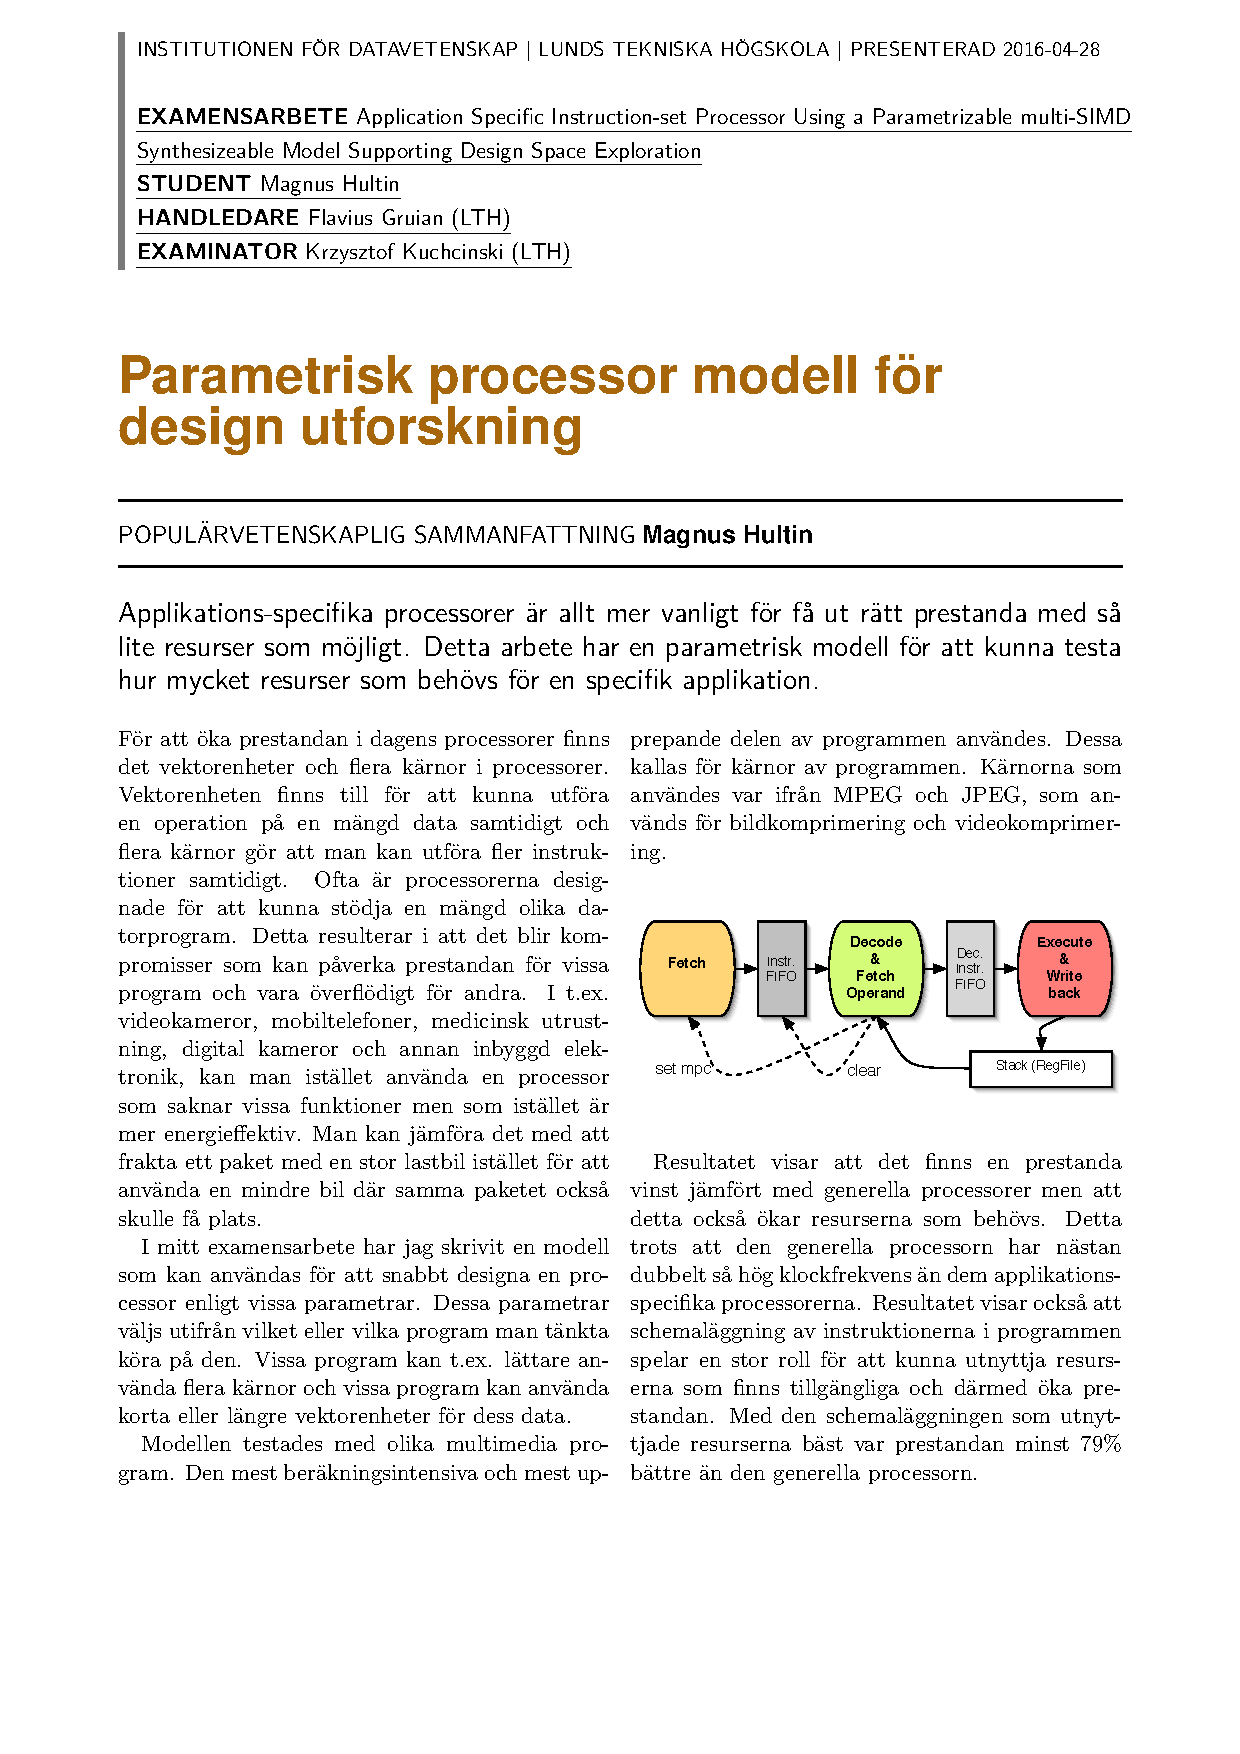
\includepdf[pages={1}]{popsci/popsci.pdf}
%\end{appendices}

\end{document}
